% =====================================================================
% Authored order dominates fixed-text entropy production:
% a measure without a zero, and a contrast without a criterion
%
% Every number in this document comes from tables/macros.tex and
% tables/tab_*.tex, which make\_tables.py generates from the measurement
% JSONs.  Do not type a figure into the prose: add it to make\_tables.py
% and reference the macro, so the text cannot drift from the data.
%
% Build:  sh build_paper.sh
% =====================================================================
\documentclass[11pt]{article}

\usepackage[utf8]{inputenc}
\usepackage[T1]{fontenc}
\usepackage{lmodern}
\usepackage[margin=1in]{geometry}
\usepackage{amsmath,amssymb,amsthm}
\usepackage{booktabs}
\usepackage{graphicx}
\usepackage{microtype}
\usepackage[hidelinks]{hyperref}
\usepackage{xcolor}

\graphicspath{{figures/}}
% generated by make_tables.py -- do not edit
\newcommand{\FbNTestsCausal}{10}
\newcommand{\FbBonferroni}{0.0050}
\newcommand{\FbNSurviving}{1}
\newcommand{\FbNNominal}{2}
\newcommand{\FbNExpected}{0.5}
\newcommand{\FbNTestsDisp}{20}
\newcommand{\FbDispPMax}{9.89\times10^{-1}}
\newcommand{\FbDispNSurviving}{11}
\newcommand{\FbAuthoredStepsBertBase}{+0.5}
\newcommand{\FbCausalStepsBertBase}{-2.5}
\newcommand{\FbAuthoredStepsLLaDA}{-6.5}
\newcommand{\FbCausalStepsLLaDA}{-0.5}
\newcommand{\FbSignPBertBase}{0.062}
\newcommand{\FbSignNegBertBase}{5/5}
\newcommand{\FbSignPLLaDA}{0.375}
\newcommand{\FbSignNegLLaDA}{4/5}
\newcommand{\TrendAuthoredRho}{+0.87}
\newcommand{\TrendAuthoredP}{0.058}
\newcommand{\TrendCausalRho}{-0.35}
\newcommand{\TrendCausalP}{0.559}
\newcommand{\TrendCeilRho}{+0.97}
\newcommand{\TrendCeilP}{0.005}
\newcommand{\TrendShareZRho}{+0.00}
\newcommand{\TrendShareZP}{1.000}
\newcommand{\TrendNEval}{5}
\newcommand{\TrendCapSpan}{32}
\newcommand{\TrendQuantum}{12}
\newcommand{\TrendCausalNDistinct}{2}
\newcommand{\TrendAuthoredNDistinct}{2}
\newcommand{\TrendCeilNDistinct}{4}
\newcommand{\TrendShareZNDistinct}{5}
\newcommand{\GridStep}{0.0417}
\newcommand{\GridK}{24}
\newcommand{\CausalCompMin}{+0.042}
\newcommand{\CausalCompMax}{+0.083}
\newcommand{\CausalCompNEval}{5}
\newcommand{\CausalCompStepsMin}{1}
\newcommand{\CausalCompStepsMax}{2}
\newcommand{\CausalCompNDistinct}{2}
\newcommand{\CausalCompCapSpan}{32}
\newcommand{\CausalCompCapLo}{124M}
\newcommand{\CausalCompCapHi}{4B}
\newcommand{\FbNCorpora}{5}
\newcommand{\FbNTexts}{2000}
\newcommand{\FbNCells}{10}
\newcommand{\FbDegenTotal}{0}
\newcommand{\FbRMin}{-0.287}
\newcommand{\FbRMax}{+0.107}
\newcommand{\FbNNegative}{9}
\newcommand{\FbMaskRateVerdict}{They agree in sign, so the reading does not depend on whether the evaluator saw the mask rates the chain rule asks it for.}
\newcommand{\FbPctCausalBertBase}{0.458}
\newcommand{\FbPctNoncausalBertBase}{0.521}
\newcommand{\FbRBertBase}{-0.126}
\newcommand{\FbAuthoredBertBase}{+0.0208}
\newcommand{\FbCausalBertBase}{-0.1042}
\newcommand{\FbPctCausalLLaDA}{0.208}
\newcommand{\FbPctNoncausalLLaDA}{0.229}
\newcommand{\FbRLLaDA}{-0.111}
\newcommand{\FbAuthoredLLaDA}{-0.2708}
\newcommand{\FbCausalLLaDA}{-0.0208}
\newcommand{\FbBetweenMin}{0.0161}
\newcommand{\FbBetweenMax}{0.1088}
\newcommand{\FbBetweenNCorpora}{5}
\newcommand{\FbBetweenCausal}{-0.0295}
\newcommand{\FbBetweenNNeg}{4}
\newcommand{\AuthoredGPTtwoMedium}{+0.354}
\newcommand{\CausalGPTtwoMedium}{+0.083}
\newcommand{\ShareGPTtwoMedium}{19}
\newcommand{\ParamsGPTtwoMedium}{355M}
\newcommand{\AuthoredGPTtwoLarge}{+0.354}
\newcommand{\CausalGPTtwoLarge}{+0.042}
\newcommand{\ShareGPTtwoLarge}{11}
\newcommand{\ParamsGPTtwoLarge}{774M}
\newcommand{\AuthoredGPTtwoXL}{+0.396}
\newcommand{\CausalGPTtwoXL}{+0.042}
\newcommand{\ShareGPTtwoXL}{10}
\newcommand{\ParamsGPTtwoXL}{1.6B}
\newcommand{\ShareZMin}{8}
\newcommand{\ShareZMax}{15}
\newcommand{\ShareZNEval}{5}
\newcommand{\MedPctCausal}{0.896}
\newcommand{\MedPctNoncausal}{0.854}
\newcommand{\PctVsNullP}{0\times10^{0}}
\newcommand{\CausalShareMedian}{12}
\newcommand{\CausalShareMin}{-5}
\newcommand{\CausalShareMax}{+40}
\newcommand{\NBlkordCells}{25}
\newcommand{\NBlocks}{4}
\newcommand{\NPerms}{24}
\newcommand{\NEval}{5}
\newcommand{\NCorp}{5}
\newcommand{\CapRatioMedian}{1.70}
\newcommand{\CapRatioMin}{1.61}
\newcommand{\CapRatioMax}{1.85}
\newcommand{\CapNCorpora}{5}
\newcommand{\CapNUp}{5}
\newcommand{\CapNSign}{0}
\newcommand{\CapDeltaLo}{+0.3469}
\newcommand{\CapDeltaHi}{+0.6140}
\newcommand{\SigmaCausal}{0.3469}
\newcommand{\AuthoredCausal}{+0.354}
\newcommand{\CausalCompCausal}{+0.042}
\newcommand{\CausalShareCausal}{11}
\newcommand{\BlkRMasked}{+0.316}
\newcommand{\BlkNSepMasked}{5}
\newcommand{\BlkNTotMasked}{5}
\newcommand{\BlkPMaxMasked}{5\times10^{-13}}
\newcommand{\BlkPctCMasked}{0.750}
\newcommand{\BlkPctNMasked}{0.500}
\newcommand{\BlkRCausal}{+0.244}
\newcommand{\BlkNSepCausal}{3}
\newcommand{\BlkNTotCausal}{5}
\newcommand{\BlkPMaxCausal}{2\times10^{-18}}
\newcommand{\BlkPctCCausal}{0.896}
\newcommand{\BlkPctNCausal}{0.854}
\newcommand{\NSepCausal}{2}
\newcommand{\NTotCausal}{5}
\newcommand{\SigTokRatioMin}{7.2}
\newcommand{\SigTokRatioMax}{10.9}
\newcommand{\NTokLarger}{5}
\newcommand{\NTokCells}{5}
\newcommand{\NTokNegAR}{3}
\newcommand{\NTokNegARTot}{5}
\newcommand{\ToyNCap}{5}
\newcommand{\ToyDMin}{32}
\newcommand{\ToyDMax}{160}
\newcommand{\ToyOrdersAbove}{17}
\newcommand{\ReproMaxErr}{8.5\times10^{-14}}
\newcommand{\ReproNCorpora}{14}
\newcommand{\AoarOrderDev}{1.8\times10^{-15}}
\newcommand{\AoarNormDev}{4.4\times10^{-16}}
\newcommand{\ARSpanRatio}{32}
\newcommand{\GapSpreadRatio}{2.0}
\newcommand{\ParamsBertBase}{110M}
\newcommand{\ParamsBertLarge}{340M}
\newcommand{\ParamsLLaDA}{8B}
\newcommand{\AuthoredGPTtwo}{+0.354}
\newcommand{\CausalGPTtwo}{+0.042}
\newcommand{\ShareGPTtwo}{11}
\newcommand{\ParamsGPTtwo}{124M}
\newcommand{\CeilGPTtwo}{32}
\newcommand{\CeilNGPTtwo}{20}
\newcommand{\AuthoredQwen}{+0.396}
\newcommand{\CausalQwen}{+0.042}
\newcommand{\ShareQwen}{10}
\newcommand{\ParamsQwen}{4B}
\newcommand{\CeilQwen}{40}
\newcommand{\CeilNQwen}{15}
\newcommand{\RGPTtwo}{+0.244}
\newcommand{\RQwen}{+0.381}
\newcommand{\GapGPTtwo}{+0.042}
\newcommand{\GapQwen}{+0.042}
\newcommand{\PctCGPTtwo}{0.896}
\newcommand{\PctCQwen}{0.938}
\newcommand{\PctNGPTtwo}{0.854}
\newcommand{\PctNQwen}{0.896}
\newcommand{\RoomGPTtwo}{0.146}
\newcommand{\RoomQwen}{0.104}
\newcommand{\RatioGPTtwo}{0.29}
\newcommand{\RatioQwen}{0.40}
\newcommand{\RatioLoGPTtwo}{0.00}
\newcommand{\RatioHiGPTtwo}{0.57}
\newcommand{\RatioLoQwen}{0.40}
\newcommand{\RatioHiQwen}{0.57}
\newcommand{\RatioMin}{0.29}
\newcommand{\RatioMax}{0.57}
\newcommand{\RatioNEval}{5}
\newcommand{\RatioNCI}{5}
\newcommand{\RatioOverlapLo}{0.40}
\newcommand{\RatioOverlapHi}{0.57}
\newcommand{\RatioWidestLo}{0.00}
\newcommand{\RatioWidestHi}{0.57}
\newcommand{\RCausal}{+0.142}
\newcommand{\ToySigmaMin}{6.28\times10^{-3}}
\newcommand{\ToySigmaMax}{2.59\times10^{-2}}
\newcommand{\ToyCapRatio}{4.1}
\newcommand{\ToySigmaAR}{4.0\times10^{-20}}
\newcommand{\ToyRmsAR}{0.0000}
\newcommand{\ToyL}{6}
\newcommand{\ToyV}{4}
\newcommand{\ToyStates}{4096}
\newcommand{\ToyN}{100{,}000}
\newcommand{\RGPTtwoMedium}{+0.265}
\newcommand{\GapGPTtwoMedium}{+0.083}
\newcommand{\PctCGPTtwoMedium}{0.938}
\newcommand{\PctNGPTtwoMedium}{0.854}
\newcommand{\RoomGPTtwoMedium}{0.146}
\newcommand{\RGPTtwoLarge}{+0.277}
\newcommand{\GapGPTtwoLarge}{+0.042}
\newcommand{\PctCGPTtwoLarge}{0.938}
\newcommand{\PctNGPTtwoLarge}{0.854}
\newcommand{\RoomGPTtwoLarge}{0.146}
\newcommand{\RGPTtwoXL}{+0.316}
\newcommand{\GapGPTtwoXL}{+0.042}
\newcommand{\PctCGPTtwoXL}{0.938}
\newcommand{\PctNGPTtwoXL}{0.896}
\newcommand{\RoomGPTtwoXL}{0.104}
\newcommand{\CausalShareNPos}{22}
\newcommand{\CausalShareNTot}{25}
\newcommand{\CeilGPTtwoMedium}{32}
\newcommand{\CeilNGPTtwoMedium}{15}
\newcommand{\RatioGPTtwoMedium}{0.57}
\newcommand{\RatioLoGPTtwoMedium}{0.29}
\newcommand{\RatioHiGPTtwoMedium}{0.57}
\newcommand{\CeilGPTtwoLarge}{33}
\newcommand{\CeilNGPTtwoLarge}{16}
\newcommand{\RatioGPTtwoLarge}{0.40}
\newcommand{\RatioLoGPTtwoLarge}{0.29}
\newcommand{\RatioHiGPTtwoLarge}{0.57}
\newcommand{\CeilGPTtwoXL}{36}
\newcommand{\CeilNGPTtwoXL}{16}
\newcommand{\RatioGPTtwoXL}{0.40}
\newcommand{\RatioLoGPTtwoXL}{0.40}
\newcommand{\RatioHiGPTtwoXL}{0.57}


% ---------------------------------------------------------------------
% Set this once the repository is public.  Leave it empty and both the
% Reproducibility section and the data-availability line say so visibly,
% rather than silently omitting the reference.
\newcommand{\repourl}{}
% e.g. \renewcommand{\repourl}{https://github.com/USER/REPO}
% ---------------------------------------------------------------------
\newcommand{\repoline}{%
  \ifx\repourl\empty
    \todo{Set \textbackslash repourl in the preamble to the public
      repository URL before submission.}%
  \else
    \url{\repourl}%
  \fi}

\newtheorem{theorem}{Theorem}
\newtheorem{proposition}[theorem]{Proposition}
\newtheorem{remark}[theorem]{Remark}

\DeclareMathOperator{\KL}{D_{\mathrm{KL}}}
\newcommand{\sigblock}{\sigma_{\mathrm{block}}}
\newcommand{\sigtok}{\sigma_{\mathrm{token}}}
\newcommand{\todo}[1]{\textcolor{red}{[#1]}}

\title{Authored order dominates fixed-text entropy production:\\
\large a measure without a zero, and a contrast without a criterion}
\author{Y.-H. Taguchi\\
\small Department of Physics, Chuo University, Tokyo, Japan\\
\small \texttt{tag.16d@g.chuo-u.ac.jp}}
\date{\today}

\begin{document}
\maketitle

\begin{abstract}
For a fixed text $x$, the quantity $\sigma = [\log P(x) - \log P(\tilde{x})]/L$
evaluated with a language model has recently been read as an entropy
production, and used to separate causally ordered prose from prose whose
sentence order is arbitrary.  We reproduce those measurements independently, to
$10^{-13}$ on the published per-text values, and then ask what the quantity is
anchored to.

The instrument is a permutation construction.  Scoring the same sentences in all
$n!$ orders yields a set of $\sigma$ values that is \emph{exactly} antisymmetric,
hence centred at zero as an identity rather than as an empirical finding; the
position of the written order within its own permutation set is then unitless,
bounded, equal to $0.50$ for any score blind to sentence order, and comparable
across scorer types that $\sigma$ itself cannot be compared across.  Each text
becomes its own control, and the measurement can be made without using the
causal labels at all.  Replacing a single reversal by the full set costs $n!$
scores instead of two and supplies the reference configuration that $\sigma$
lacks.

With it, neither reading of $\sigma$ survives.  The first result requires no
judgement about causality at all.  Taking only the texts whose sentence order is arbitrary, the
order in which they were in fact written sits far above the order-blind null
for every capable evaluator, and the size of that effect grows with evaluator
capacity: within one masked model family it runs $\AuthoredBertBase$ at
$\ParamsBertBase$, $\AuthoredBertLarge$ at $\ParamsBertLarge$ and
$\AuthoredLLaDA$ at $\ParamsLLaDA$.  An autoregressive model reaches the same
level at $\ParamsGPTtwo$ ($\AuthoredGPTtwo$), because its factorisation already
runs in the order under test.  Since $\sigma$ also has no
evaluator-independent scale --- it is not commensurable between scorer types,
it grows with capacity by a median factor of $\CapRatioMedian$ over a masked
pair and $\ToyCapRatio$ across a capacity sweep in an exactly solvable system,
and in that system, whose generating process satisfies detailed balance and so
has zero entropy production, a masked evaluator still returns a non-zero value
that does not fall with capacity --- a bare $\sigma$ cannot be read as a
quantity of causal structure.  The second result concerns the labelled contrast, and here the
limitation is not statistical.  The labels record that a language model, asked
for a passage whose sentences stand in a causal sequence, produced one; no
independent criterion is applied, and the five corpora vary the generating model
while holding that one prompt pair fixed, so their agreement rules out generator
idiosyncrasy and not construct validity.  What we can report is that $\sigma$
separates these two prompt-defined sets robustly --- in $\BlkNSepMasked$ of
$\BlkNTotMasked$ corpora at $\ParamsBertBase$ --- and that the share of
$\sigma$ attributable to that separation falls with capacity, from
$\ShareBertBase\%$ to $\ShareBertLarge\%$ within one masked family, while the
fraction of texts whose written order is already the single most costly
arrangement rises.  What we cannot report is what the separation is a separation
of.  Taken together: $\sigma$ admits no reading as a quantity, because it has no
zero, and no reading as a test for causal structure, because the contrast it
resolves has never been defined independently of the prompt that produced it.
The construction that does carry weight is the permutation set, which supplies a
zero as an identity and makes the label-free measurement possible.
\end{abstract}

% =====================================================================
\section{Introduction}

Recent work places a thermodynamic reading on a simple measurement.  Take a
fixed text $x$ of $L$ tokens, reverse it to obtain $\tilde{x}$, score both with
a language model, and form
\begin{equation}
\sigma \;=\; \frac{\log P(x) - \log P(\tilde{x})}{L} .
\label{eq:sigma}
\end{equation}
With an autoregressive evaluator this is read as an entropy production, and
$\sigma > 0$ as an arrow of time carried by the text.  The reading is supported
by a contrast between two sets of generated passages: those whose sentences
stand in a causal order, and those whose sentences are arranged arbitrarily.
The first set scores higher.

We reproduce this.  Before any of what follows, the statistical layer of the
published analysis was recomputed independently from the released per-text
values and agrees to $10^{-13}$, and every effect size and rank statistic
reported there is recovered.  Nothing below disputes a measured number.  What
we examine is what the number is anchored to.

Two questions are left open, and they are of different kinds.

The first is about the quantity.  Equation~\eqref{eq:sigma} has no zero.  It is
not comparable between a masked and an autoregressive scorer, because the two
sum conditionals over different context sets.  It is not comparable between
model sizes, since we find it grows with capacity.  And it is not anchored to
any reference configuration of the text, so there is nothing a value of
$\sigma$ can be large or small \emph{relative to}.  A quantity in that position
can still rank two groups of texts; it cannot express how much of anything a
single text has.

The second is about the labels.  The two text sets were produced by different
generation prompts, and ``causal'' there means that a language model, asked for
a passage whose sentences stand in a causal sequence, produced one.  No
independent criterion is applied --- no intervention, no counterfactual, no
specified causal structure the text is checked against.  The sets also differ
in ways other than the one of interest: in these corpora their token counts
differ significantly in four of five, and the non-causal passages are not
incoherent --- their topic continues, their pronouns resolve backwards, their
connectives are in place.  They are coherent discourse whose sentence order is
simply not causal.

This paper addresses both, and it is worth separating what each addresses.

For the first, we replace the single reversal by the full set of sentence
orders.  For a text of $n$ sentence blocks, scoring all $n!$ arrangements
yields a set of $\sigma$ values that is \emph{exactly} symmetric about zero, as
an identity rather than as a finding (Section~\ref{sec:blkord}).  That supplies
the missing reference: the position of the written order within its own
permutation set is a rank, hence unitless, bounded, comparable across scorer
types, and equal to $0.50$ for any score that cannot distinguish the
arrangements.  Each text becomes its own control.

For the second, nothing can repair labels we did not generate.  We therefore
organise the results so that the principal finding does not use them.  Our
first result is computed on the non-causal texts alone, and asks only where the
order those texts were written in sits among rearrangements of the same
sentences.  The word ``causal'' does not enter that computation.  Our second
result does use the labels, and we state its dependence on them plainly.

The findings are as follows.  Authored order --- the mere fact that a writer
settled on one arrangement --- is a large and robust signal, and the stronger
the evaluator, the more of $\sigma$ it accounts for.  The labelled contrast is a
further, smaller contribution; it is robust across evaluators, but what it is a
contrast \emph{of} is not established, and we argue in
Section~\ref{sec:construct} that no measurement on these corpora can establish
it.  The measurements we re-examine are reproduced throughout; what we dispute
is not their values but both readings placed on them --- the magnitude, which
has no zero, and the contrast, which has no criterion.

% =====================================================================
\section{Background}

\subsection{Fixed-text entropy production}
The protocol fixes the text and varies only its order.  Two reversals are used.
\emph{Token reversal} maps $x_k \mapsto x_{L+1-k}$, giving a sequence with the
same tokens and no grammar.  \emph{Block reversal} splits the text at sentence
boundaries and reverses the order of the sentences, leaving each sentence
intact.  The corresponding quantities are written $\sigtok$ and $\sigblock$.

Only the second bears on sentence order.  Token reversal destroys syntax, so the
resulting $\sigma$ is dominated by grammaticality: in our measurements it is an
order of magnitude larger than $\sigblock$ for every evaluator, and its
causal/non-causal effect size is \emph{negative} in three of five corpora for
the masked models and in two of five for the autoregressive one --- the
non-causal texts score higher.  A quantity whose sign on the contrast of
interest flips when the reversal operation is changed is not measuring that
contrast, so we follow the block-level analysis throughout and report $\sigtok$
only for completeness.

\subsection{What a reversal of a fixed text is, and is not}
A reversal in the sense of stochastic thermodynamics is a \emph{protocol}
reversal: the same dynamics run with the driving protocol time-reversed, as in
the Crooks relation.  Reversing a fixed token sequence is not that.  It asks the
model to account for the same content presented in the opposite order, which is
a question about the model's conditionals rather than about a physical process.

A related point bounds what can be expected.  For a stationary process the
Shannon entropy rate is invariant under time reversal, so a gap between the
forward and backward cross-entropy of a fixed corpus is not an informational
asymmetry in the source.  It is a property of the model and of the order in
which that model consumes its input --- which is consistent with reading
$\sigma$ as model-relative, and is one reason its dependence on the evaluator
(Section~\ref{sec:capacity}) is worth measuring rather than assuming away.

% =====================================================================
\section{Methods}
\label{sec:methods}

\subsection{Evaluators}
Five evaluators are used, spanning two model classes and a seventyfold range of
capacity within the masked class:
\begin{center}
\begin{tabular}{llll}
\toprule
model & parameters & direction & role \\
\midrule
\texttt{bert-base-uncased}    & 110M & masked & capacity series, and \\
\texttt{bert-large-uncased}   & 340M & masked & \quad matched against \texttt{gpt2} \\
\texttt{GSAI-ML/LLaDA-8B-Base} & 8B   & masked & \\
\addlinespace
\texttt{gpt2}                 & 117M & causal & matched scale and era \\
\texttt{Qwen/Qwen3-4B-Base}   & 4B   & causal & the published evaluator \\
\bottomrule
\end{tabular}
\end{center}

Two comparisons are built into this set.  \texttt{bert-base} against
\texttt{gpt2} is matched in scale and era, so a difference between them is
attributable to directionality rather than to capacity or training data.  The
three masked models form a capacity series within one class, so a trend across
them is attributable to capacity rather than to direction.  Having both is what
allows the two effects to be told apart, and we found it necessary: on the
matched pair alone the result reads as a property of the autoregressive class,
and the capacity series shows that it is not.

\subsection{Scores, and the scope of what is being measured}
\label{sec:scope}
For a causal evaluator the score is the exact $\log P(x)$, with one
beginning-of-sequence token prepended so that every content token is scored
once.  For a masked evaluator it is the pseudo-log-likelihood
$\mathrm{PLL}(x) = \sum_k \log p_\theta(x_k \mid x_{-k})$, computed with one
forward pass per masked position; the special tokens wrapping the input are
never masked and never scored.

Two consequences constrain \emph{our} instrument rather than the work we
re-examine.

First, a masked model's conditionals are in general incompatible with every
joint distribution, so for such a model there is no $P$ and the identification
$\sigma = \KL(P_{\rightarrow} \,\|\, P_{\leftarrow})$ has no referent.  This is
not an omission in the framework we build on: that framework is formulated for
autoregressive models, which do supply a factorised joint, and it never claimed
otherwise.  It is the price of leaving that class in order to ask a question the
class cannot pose.  What survives is a well-defined score difference, which is
what the questions here require.

Second, and for the same reason, $\sigma$ from a PLL and $\sigma$ from a
log-probability are \emph{not commensurable}: a PLL sums conditionals on $L-1$
tokens, an autoregressive $\log P$ sums conditionals on $k-1$ tokens.  The
medians differ accordingly, $\SigmaMasked$ against $\SigmaCausal$, and nothing
follows from their ratio.  No comparison in this paper is drawn from it; every
cross-evaluator statement rests on a rank statistic or on the permutation
decomposition below, both of which are scale-free.  This non-commensurability
is itself part of the first result: it is one of the three senses in which
$\sigma$ has no zero.

\subsection{The permutation construction, and the zero it supplies}
\label{sec:blkord}
Let the text consist of $n$ sentence blocks and let $x_\pi$ be the same blocks
concatenated in the order $\pi$.  Block reversal of $x_\pi$ is exactly
$x_{\pi\circ\mathrm{rev}}$, so for any score $S$,
\begin{equation}
\sigma(\pi) \;=\; \frac{S(x_\pi) - S(x_{\pi\circ\mathrm{rev}})}{L}
\;=\; -\,\sigma(\pi\circ\mathrm{rev}).
\label{eq:antisym}
\end{equation}
Since $\pi \mapsto \pi\circ\mathrm{rev}$ is a measure-preserving involution on
the symmetric group, the distribution of $\sigma$ over a uniformly drawn $\pi$
is \emph{exactly} symmetric about zero --- whatever the model, the text, or its
content.  This is the construction's point.  Equation~\eqref{eq:sigma} has no
reference configuration; Eq.~\eqref{eq:antisym} manufactures one, because the
set $\{\sigma(\pi)\}$ is centred at zero by identity.

Equation~\eqref{eq:antisym} also disqualifies the obvious control.  Comparing
the written order against a shuffled one compares it against the \emph{centre}
of a symmetric set, which is zero by construction; such a comparison can only
restate $\sigma(\mathrm{id}) > 0$, which is already known.  What is not forced
is the \emph{rank} of $\sigma(\mathrm{id})$ among all $n!$ orders, and that is
the statistic used here.  With $n = 4$ for every text in these corpora the
enumeration is exact rather than sampled.

The rank must split ties.  A score that cannot distinguish the block orders at
all gives $\sigma(\pi) = 0$ for every $\pi$, and a count of
$\#\{\sigma \le \sigma(\mathrm{id})\}$ would then report $n!/n! = 1.00$ ---
``the most forward-costly arrangement there is'' --- for a model that cannot
tell the arrangements apart.  The midrank
\begin{equation}
\mathrm{pct} \;=\;
\frac{\#\{\sigma < \sigma_{\mathrm{id}}\}
      + \tfrac{1}{2}\,\#\{\sigma = \sigma_{\mathrm{id}}\}}{n!}
\label{eq:midrank}
\end{equation}
puts that case at exactly $0.50$, which is the null this test reads against.
Both behaviours are verified in the accompanying self-test, which also confirms
that the permutation set is closed under reversal, that the $n!$ values of
$\sigma$ sum to zero as Eq.~\eqref{eq:antisym} requires, and that the midrank
is free to take any value in its range under an arbitrary score.

Because the comparison is within each text, length, vocabulary, style and topic
are identical across it, and the between-set differences noted in Section~1 do
not arise.

\subsection{Decomposition}
\label{sec:decomp}
The non-causal texts have a sentence order that is arbitrary but still the one
a writer settled on.  Their distance from the $0.50$ null therefore measures
what \emph{any} authored order earns; whatever the causal texts show beyond
that is what only causal order earns:
\begin{align}
\text{authored} &= \mathrm{med}\big(\mathrm{pct}_{\text{non-causal}}\big) - 0.50,
\label{eq:auth}\\
\text{causal}   &= \mathrm{med}\big(\mathrm{pct}_{\text{causal}}\big)
                 - \mathrm{med}\big(\mathrm{pct}_{\text{non-causal}}\big).
\label{eq:caus}
\end{align}
Only Eq.~\eqref{eq:caus} uses the labels.  Equation~\eqref{eq:auth} is computed
on one text set and one null, and is therefore independent of whether the
labelling of that set as ``non-causal'' is correct; all it assumes is that each
passage was written in some order, which is not a judgement.

Because the midrank is confined to a grid of width $1/n!$ and bounded above, a
strong evaluator can saturate it.  We therefore report the same decomposition
on $z = \sigma(\mathrm{id})\,/\,\mathrm{sd}\{\sigma(\pi)\}$, whose null is
$z = 0$ for the same reason and which has no ceiling, and we report directly
how often the written order is already the single most costly arrangement.

% =====================================================================
\section{Results I: authored order, without reference to causality}
\label{sec:authored}

This section uses only the texts whose sentence order is arbitrary, and the
null of Eq.~\eqref{eq:midrank}.  It makes no use of the causal labels.

\subsection{The written order is special, and increasingly so with capacity}
Table~\ref{tab:decomposition} and Figure~\ref{fig:blkord} give the position of
the written order among all orders of the same text.  Within the masked family
the authored component of Eq.~\eqref{eq:auth} runs
\begin{center}
\begin{tabular}{lrr}
\toprule
 & parameters & authored \\
\midrule
\texttt{bert-base-uncased}     & \ParamsBertBase  & \AuthoredBertBase \\
\texttt{bert-large-uncased}    & \ParamsBertLarge & \AuthoredBertLarge \\
\texttt{LLaDA-8B-Base}         & \ParamsLLaDA     & \AuthoredLLaDA \\
\bottomrule
\end{tabular}
\end{center}
--- a monotone increase.  The smallest model places the order a writer chose
indistinguishably from an arbitrary rearrangement of the same sentences; the
largest places it near the top of the permutation range.  The autoregressive
models reach that level at far smaller size, $\AuthoredGPTtwo$ already at
$\ParamsGPTtwo$ and $\AuthoredQwen$ at $\ParamsQwen$.

Two things follow.  Authored order is a real and detectable property of a
passage, not an artefact of one model class: a sufficiently capable evaluator
of either class finds it.  And an autoregressive factorisation obtains it
cheaply, because it runs in the order being tested, whereas a direction-neutral
model must acquire the same information from scale --- about seventy times as
much of it in this series.

We note that the first of these corrects a reading we initially drew from the
matched pair alone, where \texttt{bert-base}'s $\AuthoredBertBase$ against
\texttt{gpt2}'s $\AuthoredGPTtwo$ suggests a property of the autoregressive
class.  The capacity series is what distinguishes a class effect from a
capability effect, and it was needed.

\begin{table}[t]
\centering
% generated by make_tables.py -- do not edit
\begin{tabular}{llrrrrrr}
\toprule
 & & \multicolumn{3}{c}{midrank} & \multicolumn{3}{c}{$z$} \\
\cmidrule(lr){3-5}\cmidrule(lr){6-8}
evaluator & direction & authored & causal & share & authored & causal & share \\
\midrule
gpt2 & AR & $+0.354$ & $+0.042$ & 11\% & $+1.254$ & $+0.228$ & 15\% \\
gpt2-medium & AR & $+0.354$ & $+0.083$ & 19\% & $+1.342$ & $+0.122$ & 8\% \\
gpt2-large & AR & $+0.354$ & $+0.042$ & 11\% & $+1.330$ & $+0.151$ & 10\% \\
gpt2-xl & AR & $+0.396$ & $+0.042$ & 10\% & $+1.334$ & $+0.199$ & 13\% \\
Qwen3-4B-Base & AR & $+0.396$ & $+0.042$ & 10\% & $+1.330$ & $+0.208$ & 14\% \\
\bottomrule
\end{tabular}

\caption{Decomposition of the within-text distance from the $0.50$ null into
the component any authored order earns (Eq.~\ref{eq:auth}; computed without
reference to the causal labels) and the component only causal order earns
(Eq.~\ref{eq:caus}). Each entry is the median over five corpora of the
per-corpus quantity, so the two components are paired within a corpus and need
not sum to the median total; a share above $100\%$ means the authored component
is slightly negative. Reported in midrank units and in
$z = \sigma(\mathrm{id})/\mathrm{sd}\{\sigma(\pi)\}$, which has no ceiling: their
agreement is what shows the midrank bound is not driving the split.}
\label{tab:decomposition}
\end{table}

\begin{figure}[t]
\centering
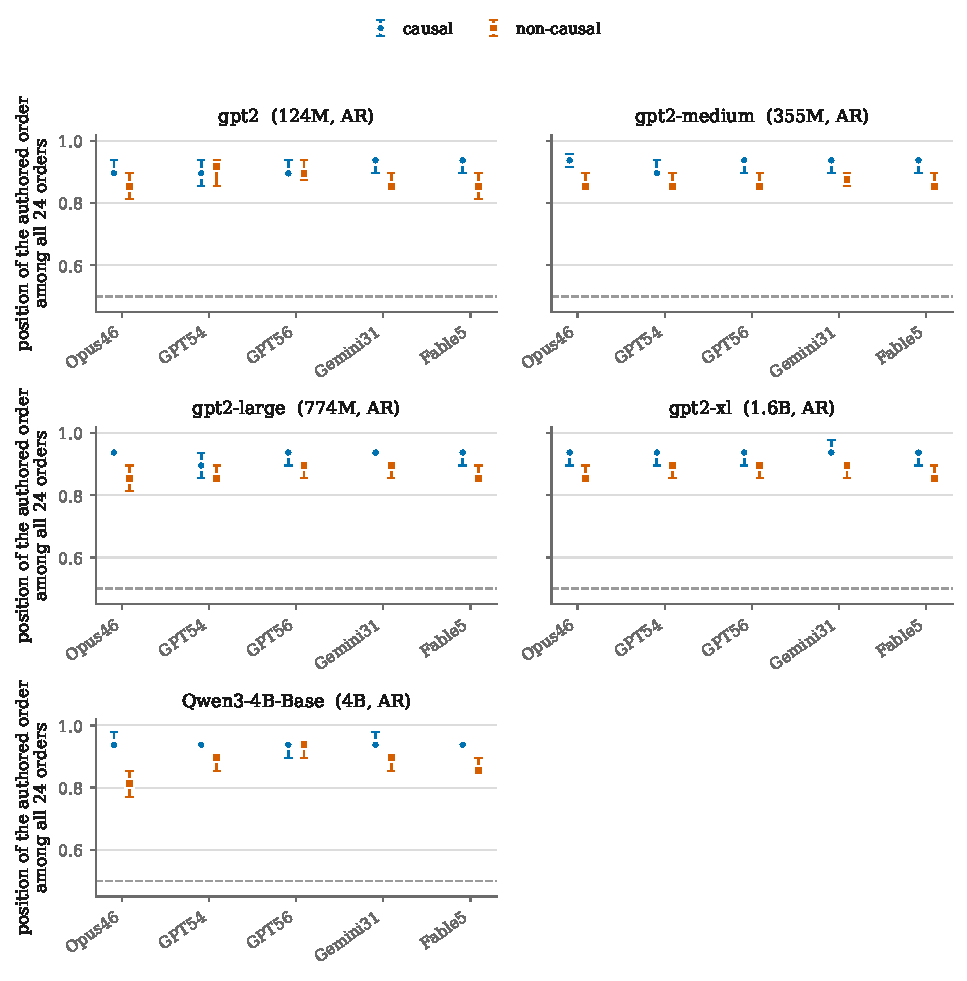
\includegraphics[width=\textwidth]{fig1_block_order.pdf}
\caption{Where the written order sits among all orders of the same text, by
evaluator in order of capacity. The dashed line at $0.50$ is the null: a score
that cannot distinguish the arrangements of a text lands there exactly. The
non-causal series is the one Section~\ref{sec:authored} reads --- it moves from
that null to near the ceiling as capacity rises --- and it does so in both model
classes, reaching the level of a $117\,\mathrm{M}$ autoregressive model only at
$8\,\mathrm{B}$ parameters without one. Bars are bootstrap $95\%$ intervals of
the median.}
\label{fig:blkord}
\end{figure}

\subsection{$\sigma$ has no zero}
\label{sec:capacity}
Three independent senses, none of which involves the labels.

\emph{It is not comparable between scorer types.}  Section~\ref{sec:scope}:
a PLL and a log-probability sum different conditionals, and the medians differ
by more than an order of magnitude for that reason alone.

\emph{It is not comparable between capacities.}  From \texttt{bert-base} to
\texttt{bert-large}, $\sigma$ grows in $\CapNUp$ of $\CapNCorpora$ corpora by a
median factor of $\CapRatioMedian$ (range $\CapRatioMin$ to $\CapRatioMax$).
The same direction appears in the exactly solvable system of
Section~\ref{sec:toy}, where $\sigma$ grows by $\ToyCapRatio$ over $\ToyNCap$
model sizes from $d = \ToyDMin$ to $d = \ToyDMax$.  A larger model has sharper
conditionals and penalises an unnatural arrangement more heavily, so $\sigma$
scales with the evaluator's confidence.

\emph{It is not anchored for a single text.}  Equation~\eqref{eq:sigma} offers
no reference arrangement.  The permutation construction supplies one, and the
remainder of this paper uses it; without it, a value of $\sigma$ is large or
small relative to nothing.

\subsection{An exactly solvable counterexample}
\label{sec:toy}
To see what a masked evaluator reports when the truth is known, we construct a
system in which $\sigma$ is computed exactly rather than estimated: a dense
pairwise Markov random field on $L = \ToyL$ sites with $V = \ToyV$ symbols,
whose $\ToyStates$ states can be enumerated.  The field is symmetric and at
equilibrium, so the generating process satisfies detailed balance and its
entropy production is \emph{zero by construction}.  Models are trained on
$N = \ToyN$ samples and the entropy production of the induced chain is obtained
from Schnakenberg network theory, with cycle affinities computed directly.

The autoregressive model recovers the truth: $\sigma = \ToySigmaAR$, machine
zero, with root-mean-square cycle affinity $\ToyRmsAR$ exactly
(Table~\ref{tab:capacity}).  The masked model does not: it returns
$\ToySigmaMin$ to $\ToySigmaMax$, eighteen orders of magnitude larger, and the
value does not fall as capacity rises.  This is a statement about the masked
instrument, and it is the reason the text results rest on within-text ranks ---
where such a floor cancels between the permutations of one text --- rather than
on the magnitude of $\sigma$.

\begin{figure}[t]
\centering
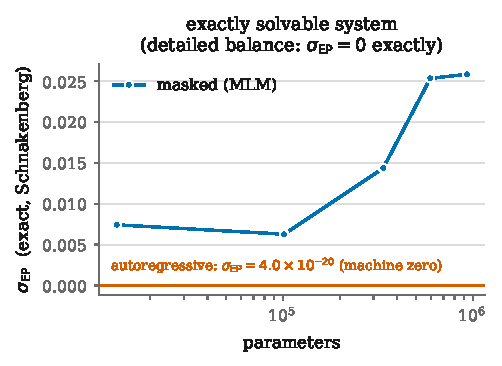
\includegraphics[width=\textwidth]{fig2_capacity.pdf}
\caption{$\sigma$ rises with evaluator capacity. Left: the exactly solvable
system, whose generating process satisfies detailed balance, so the true
entropy production is zero; the autoregressive value is stated on the zero line,
where it sits to twenty significant figures. Right: the masked pair on the
fixed texts.}
\label{fig:capacity}
\end{figure}

\begin{table}[t]
\centering
% generated by make_tables.py -- do not edit
\begin{tabular}{lrrrrr}
\toprule
model & $d$ & params & loss & $\sigma_{\mathrm{EP}}$ & $\mathrm{rms}|A|$ \\
\midrule
MLM & 32 & 13317 & 1.1148 & 0.0074 & 0.3377 \\
MLM & 64 & 101189 & 1.1286 & 0.0063 & 0.3618 \\
MLM & 96 & 337349 & 1.1360 & 0.0144 & 0.4960 \\
MLM & 128 & 597253 & 1.1430 & 0.0253 & 0.6496 \\
MLM & 160 & 930885 & 1.1570 & 0.0259 & 0.6392 \\
AR & 32 & 13317 & 1.1955 & $3.99\times10^{-20}$ & 0.0000 \\
\bottomrule
\end{tabular}

\caption{Capacity sweep in the exactly solvable system
($L = \ToyL$, $V = \ToyV$, $\ToyStates$ states, $N = \ToyN$). The generating
process is a symmetric pairwise Markov random field at equilibrium, so its
entropy production is zero by construction.}
\label{tab:capacity}
\end{table}

% =====================================================================
\section{Results II: the labelled contrast}
\label{sec:causal}

\subsection{What the labels record, and what they do not}
\label{sec:construct}
Everything in this section uses the causal/non-causal labels, so it is worth
being exact about what those labels are.

They record that a language model, given a prompt asking for a short passage
whose sentences stand in a causal sequence, produced one; and that the same
model, given a prompt asking for a passage whose sentences are arranged
arbitrarily, produced the other.  That is the entire basis.  No operational
definition of causal dependence is applied at any point.  Nothing is
intervened on, no counterfactual is evaluated, and the passages are not checked
against any specified causal structure.  ``Causal'' here is the name of a
prompt, not the result of a measurement.

Two features of the corpus design are easy to mistake for validation and are
not.

First, the five corpora were generated by five different models.  Their
agreement therefore rules out an idiosyncrasy of one generator.  It does not
bear on construct validity at all, because the \emph{prompt pair is the
constant across all five} --- what varies is the generator, not the definition.
Five applications of one undefined construct do not define it.

Second, our within-text design removes the length, vocabulary, style and topic
differences that separate the two sets, but it removes them \emph{within} a
text, across its permutations.  The comparison between the sets still runs
between texts written to different prompts.  Anything those prompts induced
systematically --- connective density, register, clause structure, sentence
length profile --- remains available to $\sigma$ and is indistinguishable from
causal order in these data.

The consequence is not that the contrast is spurious.  It is that the contrast
has no established referent: $\sigma$ separates two sets of texts, and what
distinguishes those sets is unknown.  An effect size, however large and however
stable, cannot supply the missing construct.  We therefore report the contrast
as a contrast between prompt-defined sets and nowhere describe it as a
measurement of causality.

A text set generated from an explicitly specified causal structure --- a graph
fixed in advance, with the ordering determined by that graph and not by a
prompt --- would supply the construct and make the question answerable.  We
regard that as the experiment this one points to.

\subsection{The contrast is robust across evaluators}
Within text, passages from the causally prompted set sit above those from the
arbitrarily prompted set.  The effect size reaches $|r| > 0.2$ in
$\BlkNSepMasked$ of $\BlkNTotMasked$ corpora for \texttt{bert-base}
(median $r = \BlkRMasked$) and $\BlkNSepCausal$ of $\BlkNTotCausal$ for
\texttt{gpt2} (median $r = \BlkRCausal$); Table~\ref{tab:blkord} gives every
cell.  The separation does not decay with capacity, and it appears in both
model classes.

By Section~\ref{sec:construct} this robustness is evidence that the two
prompt-defined sets differ reliably in something $\sigma$ detects.  It is not
evidence about what that something is, and in particular it is not evidence
that a different definition of causal ordering --- temporal sequence,
interventional dependence, the presence of causal connectives --- would
reproduce it.  Those definitions would yield different text sets and are not
tested here.

\begin{table}[t]
\centering
% generated by make_tables.py -- do not edit
\begin{tabular}{llrrrrr}
\toprule
evaluator & corpus & $n$ & causal & non-causal & $r$ & $p$ \\
\midrule
bert-base-uncased (110M, masked) & Opus46 & 200 & 0.729 & 0.479 & +0.927 & $7\times10^{-30}$ \\
 & GPT54 & 200 & 0.729 & 0.479 & +0.898 & $4\times10^{-28}$ \\
 & GPT56 & 200 & 0.729 & 0.479 & +0.910 & $7\times10^{-29}$ \\
 & Gemini31 & 200 & 0.771 & 0.521 & +0.897 & $4\times10^{-28}$ \\
 & Fable5 & 200 & 0.771 & 0.479 & +0.903 & $2\times10^{-28}$ \\
\addlinespace
gpt2 (117M, causal) & Opus46 & 200 & 0.896 & 0.812 & +0.303 & $2\times10^{-4}$ \\
 & GPT54 & 200 & 0.896 & 0.854 & +0.338 & $3\times10^{-5}$ \\
 & GPT56 & 200 & 0.896 & 0.854 & +0.242 & $0.003$ \\
 & Gemini31 & 200 & 0.896 & 0.854 & +0.336 & $3\times10^{-5}$ \\
 & Fable5 & 200 & 0.896 & 0.854 & +0.253 & $0.002$ \\
\addlinespace
bert-large-uncased (340M, masked) & Opus46 & 200 & 0.771 & 0.562 & +0.852 & $1\times10^{-25}$ \\
 & GPT54 & 200 & 0.771 & 0.562 & +0.826 & $4\times10^{-24}$ \\
 & GPT56 & 200 & 0.771 & 0.562 & +0.881 & $3\times10^{-27}$ \\
 & Gemini31 & 200 & 0.771 & 0.562 & +0.806 & $5\times10^{-23}$ \\
 & Fable5 & 200 & 0.771 & 0.562 & +0.814 & $2\times10^{-23}$ \\
\addlinespace
Qwen3-4B-Base (4B, causal) & Opus46 & 200 & 0.938 & 0.938 & +0.131 & $0.100$ \\
 & GPT54 & 200 & 0.938 & 0.896 & +0.232 & $0.004$ \\
 & GPT56 & 200 & 0.958 & 0.896 & +0.302 & $1\times10^{-4}$ \\
 & Gemini31 & 200 & 0.958 & 0.896 & +0.308 & $1\times10^{-4}$ \\
 & Fable5 & 200 & 0.938 & 0.896 & +0.120 & $0.127$ \\
\addlinespace
LLaDA-8B-Base (8B, masked) & Opus46 & 200 & 0.958 & 0.854 & +0.496 & $5\times10^{-10}$ \\
 & GPT54 & 200 & 0.938 & 0.854 & +0.405 & $5\times10^{-7}$ \\
 & GPT56 & 200 & 0.979 & 0.854 & +0.550 & $7\times10^{-12}$ \\
 & Gemini31 & 200 & 0.938 & 0.854 & +0.563 & $2\times10^{-12}$ \\
 & Fable5 & 200 & 0.938 & 0.854 & +0.541 & $2\times10^{-11}$ \\
\bottomrule
\end{tabular}

\caption{Position of the written sentence order among all $4!$ orders of the
same text, as the midrank of Eq.~\eqref{eq:midrank}; $0.50$ is where a score
blind to sentence order lands.}
\label{tab:blkord}
\end{table}

\subsection{The share falls, and the room runs out}
\label{sec:window}
Two trends run against each other.  The causal component of
Eq.~\eqref{eq:caus} is stable or growing in absolute terms, but the authored
component grows faster, so the share of the measured distance attributable to
causal order falls with capacity: $\ShareBertBase\%$ at $\ParamsBertBase$,
$\ShareBertLarge\%$ at $\ParamsBertLarge$, $\ShareLLaDA\%$ at $\ParamsLLaDA$.
The autoregressive evaluators, which reach the authored level early, sit at
$\ShareGPTtwo\%$ and $\ShareQwen\%$.

The fall is not an artefact of the midrank's ceiling: the same ordering appears
in the $z$ decomposition, which is unbounded above
(Table~\ref{tab:decomposition}).  But a ceiling is approaching all the same, and
it is a ceiling in the phenomenon rather than in the statistic.  Once the
written order \emph{is} the single most costly arrangement, no normalisation can
express a further increase.  Table~\ref{tab:saturation} reports how often that
has already happened: for causally labelled texts it rises to $\CeilQwen\%$ and
$\CeilLLaDA\%$ at the largest evaluators, against $\CeilBertLarge\%$ at
$\ParamsBertLarge$.

The protocol therefore has a capability window.  Below it an evaluator cannot
detect authored order at all, and the decomposition degenerates --- which is
what \texttt{bert-base}'s $\ShareBertBase\%$ causal share reflects, a failure
to detect the denominator rather than a purity of the numerator.  Above it the
written order becomes the argmax for a large fraction of texts and the measure
loses resolution.  We do not extrapolate past $\ParamsLLaDA$; what the data
support is that the room is shrinking monotonically and is already half gone at
that size.

\begin{table}[t]
\centering
% generated by make_tables.py -- do not edit
\begin{tabular}{llrrrrr}
\toprule
 & & & \multicolumn{2}{c}{at ceiling} & & gap / room \\
\cmidrule(lr){4-5}
evaluator & direction & params & causal & non-causal & gap & (95\% CI) \\
\midrule
bert-base-uncased & masked & 110M & 13\% & 4\% & $+0.208$ & 0.43  [0.30, 0.57] \\
gpt2 & AR & 124M & 32\% & 20\% & $+0.042$ & 0.29  [0.00, 0.57] \\
bert-large-uncased & masked & 340M & 17\% & 6\% & $+0.208$ & 0.48  [0.35, 0.61] \\
gpt2-medium & AR & 355M & 32\% & 15\% & $+0.083$ & 0.57  [0.29, 0.57] \\
gpt2-large & AR & 774M & 33\% & 16\% & $+0.042$ & 0.40  [0.29, 0.57] \\
gpt2-xl & AR & 1B & 36\% & 16\% & $+0.042$ & 0.40  [0.40, 0.57] \\
Qwen3-4B-Base & AR & 4B & 40\% & 15\% & $+0.042$ & 0.40  [0.40, 0.57] \\
LLaDA-8B-Base & masked & 8B & 47\% & 18\% & $+0.083$ & 0.57  [0.40, 0.80] \\
\bottomrule
\end{tabular}

\caption{Fraction of texts whose written order is the single most
forward-costly of all $4!$ arrangements. Once a text is at this ceiling the
measure has no room above it, for any normalisation. Medians over five
corpora.}
\label{tab:saturation}
\end{table}

\subsection{The between-set measurement}
The same ordering appears in the original between-set protocol
(Table~\ref{tab:pll}): the masked evaluator separates the sets in
$\NSepMasked$ of $\NTotMasked$ corpora with median $r = \RMasked$, the
matched-scale autoregressive one in $\NSepCausal$ of $\NTotCausal$ with
$r = \RCausal$, and raising capacity within the masked family gives
$r = \RMaskedLarge$ in $\NSepMaskedLarge$ of $\NTotMaskedLarge$.  We draw no
conclusion from the $\sigma$ column across scorer types
(Section~\ref{sec:scope}).

\begin{table}[t]
\centering
% generated by make_tables.py -- do not edit
\begin{tabular}{llrrrr}
\toprule
evaluator & corpus & $n$ & median $\Delta_{\mathrm{block}}$ & $r$ & $p$ \\
\midrule
bert-base-uncased (110M, masked) & Opus46 & 200 & 0.0235 & +0.584 & $1\times10^{-12}$ \\
 & GPT54 & 200 & 0.0218 & +0.352 & $2\times10^{-5}$ \\
 & GPT56 & 200 & 0.0213 & +0.319 & $1\times10^{-4}$ \\
 & Gemini31 & 200 & 0.0103 & +0.203 & $0.013$ \\
 & Fable5 & 200 & 0.0242 & +0.338 & $4\times10^{-5}$ \\
\addlinespace
gpt2 (124M, AR) & Opus46 & 200 & 0.3182 & +0.523 & $2\times10^{-10}$ \\
 & GPT54 & 200 & 0.4216 & -0.007 & $0.935$ \\
 & GPT56 & 200 & 0.3468 & -0.163 & $0.046$ \\
 & Gemini31 & 200 & 0.3676 & +0.207 & $0.011$ \\
 & Fable5 & 200 & 0.3469 & +0.142 & $0.083$ \\
\addlinespace
bert-large-uncased (340M, masked) & Opus46 & 200 & 0.0487 & +0.515 & $3\times10^{-10}$ \\
 & GPT54 & 200 & 0.0302 & +0.513 & $4\times10^{-10}$ \\
 & GPT56 & 200 & 0.0262 & +0.243 & $0.003$ \\
 & Gemini31 & 200 & 0.0243 & +0.297 & $3\times10^{-4}$ \\
 & Fable5 & 200 & 0.0433 & +0.424 & $2\times10^{-7}$ \\
\bottomrule
\end{tabular}

\caption{Block-level $\sigma$ and the causal/non-causal effect size for each
evaluator in the original between-set protocol. The $\sigma$ column is in each
evaluator's own units of account and is not comparable across scorer types.}
\label{tab:pll}
\end{table}

\begin{figure}[t]
\centering
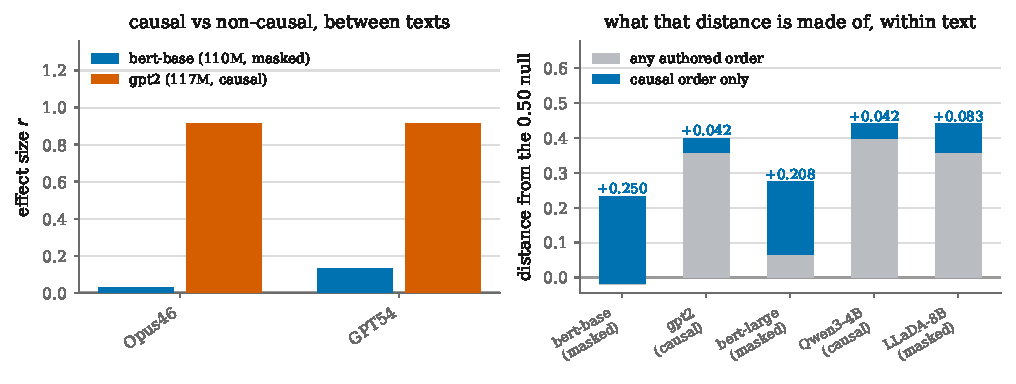
\includegraphics[width=\textwidth]{fig3_evaluators.pdf}
\caption{Left: the causal/non-causal effect size by corpus and evaluator in the
original between-set protocol, a rank statistic and therefore comparable across
scorer types; this protocol was run for the three smaller evaluators. Right: the
decomposition of Section~\ref{sec:decomp}, for all five. The grey component is
measured on the non-causal texts alone and uses no causal judgement.}
\label{fig:evaluators}
\end{figure}

% =====================================================================
\section{Discussion}

Our conclusion is negative in two independent ways, and the two should not be
conflated.

As a \emph{quantity}, $\sigma$ cannot be interpreted, and the reasons are
structural rather than statistical.  It has no zero in three independent senses
(Section~\ref{sec:capacity}).  Most of its magnitude is attributable to the bare
fact that a writer settled on an order, and that fraction grows with the
capability of the evaluator.  The construction that does supply a zero, the
permutation set, is approaching its own ceiling at current model sizes.  All of
this is established without reference to any judgement about causality.

As a \emph{test for causal structure}, $\sigma$ is not evaluable on these
corpora at all.  It does separate the two prompt-defined sets, robustly and
across evaluator classes; but the sets were never characterised except by the
prompt that produced them, so the separation has no established referent.  This
is not a weakness of the statistic.  It is a missing construct, and no
refinement of the measurement supplies one.

The practical consequences are narrow and concrete.  A value of $\sigma$ should
not be quoted for a text, or compared between models.  Where a reference is
needed, the permutation set of the text itself supplies one that is unitless and
model-independent, at a cost of $n!$ scores rather than two.  An evaluator should
be chosen inside the capability window of Section~\ref{sec:window}, with both
ends checked rather than assumed.  And a contrast between text sets should not
be reported as a measurement of a property those sets were never shown to
differ in.

Finally, on scope.  The framework these measurements belong to is built for
autoregressive models, and the quantity it defines requires a factorised joint,
which masked models do not supply.  Our use of masked evaluators is a probe from
outside that framework, purchased at the cost of the divergence interpretation.
That the probe reproduces the framework's empirical claim while showing its
central quantity to be unanchored seems to us the most useful thing such a probe
can do.

% =====================================================================
\section{Limitations}
\label{sec:limitations}

\emph{The labels.}  Treated in Section~\ref{sec:construct} rather than here,
because it is not a caveat on the result but a limit on what the result can be
about.  Section~\ref{sec:authored} is constructed to be independent of the
labels; Section~\ref{sec:causal} is not, and no measurement on these corpora
can make it so.

\emph{The authored component is not decomposed.}  The non-causal passages are
coherent discourse, so what we call authored order mixes topical continuity,
anaphoric dependence and given--new ordering.  Separating these would need text
sets built for the purpose.

\emph{The masked floor is characterised only in the exactly solvable system.}
Two controls on text remain: a corpus of sentences drawn from unrelated
documents, which removes topical continuity, and a word-shuffled corpus, which
removes syntax as well.  Their $\sigma$ would bound the part of the masked
measurement that no ordering of the content can explain.

\emph{Enumeration.}  Every text here has exactly four sentence blocks, so the
$4! = 24$ enumeration is exact.  Longer texts require sampling the permutation
set, and the sampled set must be closed under reversal for
Eq.~\eqref{eq:antisym} to hold.

\emph{The pseudo-log-likelihood is not a log-probability}
(Section~\ref{sec:scope}).  The any-order chain rule of a masked diffusion model
does give one, at the price of a free unmasking order with no counterpart in the
physics.  The two instruments answer different questions.

\emph{No extrapolation.}  The trends in Section~\ref{sec:window} are monotone
over the range measured and we state them as such.  Whether the causal share
continues to fall, and whether saturation becomes total, is not something this
data settles.

% =====================================================================
\section*{Reproducibility}

All code and all measured values are available at \repoline, including the
per-text JSON behind every table, the self-tests described below, and the
scripts that build this document.  The same files are attached to this
submission as ancillary material.

Every number in this paper, in the tables and in the running text alike, is
generated by \texttt{make\_tables.py} from the measurement JSON files, and every
figure by \texttt{make\_figures.py}; no figure is typed into the source, so
rerunning the measurements regenerates the prose.

The measurement scripts carry self-tests that run without model weights.  For
the any-order machinery these verify order-independence of the chain rule to
$1.8\times10^{-15}$ and normalisation to $4.4\times10^{-16}$.  For the
permutation test they verify that the permutation set is closed under reversal,
that the $n!$ values of $\sigma$ sum to zero, that the midrank is free to take
any value in its range under an arbitrary score, and --- the check that matters
most --- that an order-blind score yields a midrank of exactly $0.50$ while a
naive $\le$ count would yield $1.00$.  The statistical layer of the work we
build on is reproduced independently to $10^{-13}$ before any of the above is
run.

\todo{One item left. The titles, authors and arXiv identifiers of
Refs.~\cite{sagawa2026}, \cite{rectangle} and \cite{arrow} have been checked
against the arXiv records. The \emph{journal} reference for
Ref.~\cite{sagawa2026} (PRX Intelligence 1, 023013) does not yet appear on its
arXiv abstract page and was taken from the funding agency's press release;
confirm the volume and article number against the journal before submission.}

\bibliographystyle{unsrt}
\begin{thebibliography}{9}
\bibitem{sagawa2026}
T. Sagawa,
\emph{Stochastic Thermodynamics for Autoregressive Generative Models: A
Non-Markovian Perspective},
PRX Intelligence \textbf{1}, 023013 (2026); arXiv:2604.07867.

\bibitem{rectangle}
S. Sana, S. Wolf, N. Mehta, A. Shah, A. Shaikh, J. Goodman, L. Levine,
\emph{Mixing Times of Glauber Dynamics on Masked Language Models},
arXiv:2605.16378 (2026).

\bibitem{arrow}
V. Papadopoulos, J. Wenger, C. Hongler,
\emph{Arrows of Time for Large Language Models},
arXiv:2401.17505 (2024).

\bibitem{llada}
S. Nie et al., \emph{Large Language Diffusion Models}, arXiv:2502.09992.

\bibitem{bert}
J. Devlin, M.-W. Chang, K. Lee, K. Toutanova,
\emph{BERT: Pre-training of Deep Bidirectional Transformers for Language
Understanding}, NAACL-HLT (2019).

\bibitem{gpt2}
A. Radford et al., \emph{Language Models are Unsupervised Multitask Learners},
OpenAI technical report (2019).

\bibitem{qwen3}
Qwen Team, \emph{Qwen3 Technical Report} (2025).

\bibitem{schnakenberg}
J. Schnakenberg, \emph{Network theory of microscopic and macroscopic behavior
of master equation systems}, Rev. Mod. Phys. \textbf{48}, 571 (1976).
\end{thebibliography}

\end{document}
